\documentclass[hidelinks,12pt]{article}
\usepackage[left=0.25cm,top=1cm,right=0.25cm,bottom=1cm]{geometry}
%\usepackage[landscape]{geometry}
\textwidth = 20cm
\hoffset = -1cm
\usepackage[utf8]{inputenc}
\usepackage[spanish,es-tabla, es-lcroman]{babel}
\usepackage[autostyle,spanish=mexican]{csquotes}
\usepackage[tbtags]{amsmath}
\usepackage{nccmath}
\usepackage{amsthm}
\usepackage{amssymb}
\usepackage{mathrsfs}
\usepackage{graphicx}
\usepackage{subfig}
\usepackage{caption}
%\usepackage{subcaption}
\usepackage{standalone}
\usepackage[outdir=./Imagenes/]{epstopdf}
\usepackage{siunitx}
\usepackage{physics}
\usepackage{color}
\usepackage{float}
\usepackage{hyperref}
\usepackage{multicol}
\usepackage{multirow}
%\usepackage{milista}
\usepackage{anyfontsize}
\usepackage{anysize}
%\usepackage{enumerate}
\usepackage[shortlabels]{enumitem}
\usepackage{capt-of}
\usepackage{bm}
\usepackage{mdframed}
\usepackage{relsize}
\usepackage{placeins}
\usepackage{empheq}
\usepackage{cancel}
\usepackage{pdfpages}
\usepackage{wrapfig}
\usepackage[flushleft]{threeparttable}
\usepackage{makecell}
\usepackage{fancyhdr}
\usepackage{tikz}
\usepackage{bigints}
\usepackage{menukeys}
\usepackage{tcolorbox}
\tcbuselibrary{breakable}
\usepackage{scalerel}
\usepackage{pgfplots}
\usepackage{pdflscape}
\pgfplotsset{compat=1.16}
\spanishdecimal{.}
\renewcommand{\baselinestretch}{1.5} 
\renewcommand\labelenumii{\theenumi.{\arabic{enumii}})}

\newcommand{\python}{\texttt{python}}
\newcommand{\textoazul}[1]{\textcolor{blue}{#1}}
\newcommand{\azulfuerte}[1]{\textcolor{blue}{\textbf{#1}}}
\newcommand{\funcionazul}[1]{\textcolor{blue}{\textbf{\texttt{#1}}}}

\newcommand{\pderivada}[1]{\ensuremath{{#1}^{\prime}}}
\newcommand{\sderivada}[1]{\ensuremath{{#1}^{\prime \prime}}}
\newcommand{\tderivada}[1]{\ensuremath{{#1}^{\prime \prime \prime}}}
\newcommand{\nderivada}[2]{\ensuremath{{#1}^{(#2)}}}


\newtheorem{defi}{{\it Definición}}[section]
\newtheorem{teo}{{\it Teorema}}[section]
\newtheorem{ejemplo}{{\it Ejemplo}}[section]
\newtheorem{propiedad}{{\it Propiedad}}[section]
\newtheorem{lema}{{\it Lema}}[section]
\newtheorem{cor}{Corolario}
\newtheorem{ejer}{Ejercicio}[section]

\newlist{milista}{enumerate}{2}
\setlist[milista,1]{label=\arabic*)}
\setlist[milista,2]{label=\arabic{milistai}.\arabic*)}
\newlength{\depthofsumsign}
\setlength{\depthofsumsign}{\depthof{$\sum$}}
\newcommand{\nsum}[1][1.4]{% only for \displaystyle
    \mathop{%
        \raisebox
            {-#1\depthofsumsign+1\depthofsumsign}
            {\scalebox
                {#1}
                {$\displaystyle\sum$}%
            }
    }
}
\def\scaleint#1{\vcenter{\hbox{\scaleto[3ex]{\displaystyle\int}{#1}}}}
\def\scaleoint#1{\vcenter{\hbox{\scaleto[3ex]{\displaystyle\oint}{#1}}}}
\def\scaleiiint#1{\vcenter{\hbox{\scaleto[3ex]{\displaystyle\iiint}{#1}}}}
\def\bs{\mkern-12mu}

\newcommand{\Cancel}[2][black]{{\color{#1}\cancel{\color{black}#2}}}



\author{M. en C. Gustavo Contreras Mayén. \texttt{gux7avo@ciencias.unam.mx}}
\title{\vspace*{-3cm}Revisión de los problemas 6 y 7 del Examen Final \\ {\large Curso Física Computacional}}
\date{ }
\begin{document}

\maketitle
\fontsize{14}{14}\selectfont

\Large{Mayorquin Galicia Antonio.}

\section{Problema 6.}

\begin{enumerate}
\item En el desarrollo que planteas, propones que $\lambda$ sea de la forma:
\begin{figure}[H]
    \centering
    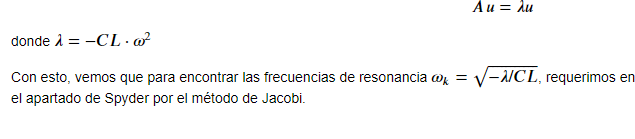
\includegraphics[scale=0.8]{Evidencia_Problema_06_01.png}
\end{figure}
pero sabemos que:
\begin{enumerate}
\item $\lambda$ son valores positivos.
\item $L$ es siempre positivo.
\item $C$ es siempre positivo.
\end{enumerate}
Por lo tanto, el que propongas la raíz cuadrada de un valor negativo, no tiene sentido físico ni matemático.
\item El uso de la función $\texttt{jacobi}$ del \texttt{moduloMatrices} es directo, devolviendo los eigenvalores y a partir de los cuales, se obtienen las frecuencias angulares pedidas en el enunciado:
{\fontsize{12}{12}\selectfont
\begin{verbatim}
Eigenvalores del sistema: 
[ 0.90516148  3.38984838  7.06445882 12.64053133]

Frecuencias angulares (unidades de 1/sqrt(LC)):
[0.95139975 1.84115409 2.65790497 3.55535249]
\end{verbatim}
}
\item El definir debidamente la matriz de coeficientes del sistema es el punto clave para que el ejercicio llevará una buena solución, un problema de este tipo ya deja de ser un enunciado matemático al que haya que darle solución directa con los algoritmos que se revisaron. Es quizá la parte más relevante de la solución, entender la congruencia con el fenómenos (es decir, con la física involucrada) de todo el procedimiento. Como lo mencioné previamente, si obtenías eigenvalores negativos, ya era un claro aviso de que algo no iba bien.
\item En tu código si se multiplica por $-1$ la matriz de coeficientes, se obtiene:
\begin{figure}[H]
    \centering
    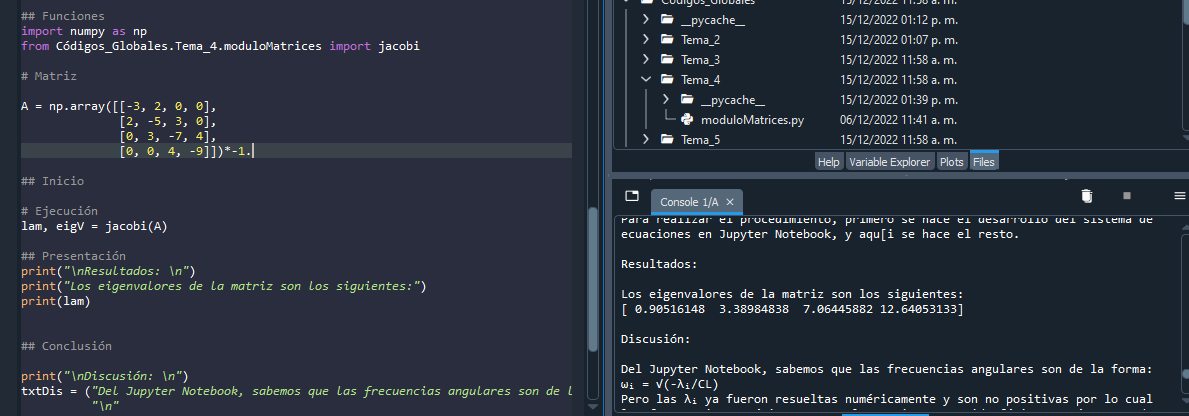
\includegraphics[scale=0.5]{Evidencia_Problema_06_02.png}
\end{figure}
\item Con lo anterior, se pone de manifiesto que la función \texttt{jacobi} opera debidamente.
\end{enumerate}

\section{Problema 7.}

\begin{enumerate}
\item Con el uso de la ley de Kirchhoff para la corriente se tiene que las corrientes en cada malla son:
\begin{align*}
2 L \dv[2]{i_{1}}{t} - L \dv{i_{2}}{t} + \dfrac{1}{C} i_{1} &= 0 \\
- L \dv[2]{i_{1}}{t} + 2 L \dv{i_{2}}{t} - L \dv[2]{i_{3}}{t} +  \dfrac{2}{C} i_{2} &= 0 \\
- L \dv[2]{i_{2}}{t} + 2 L \dv{i_{3}}{t} - L \dv[2]{i_{4}}{t} +  \dfrac{3}{C} i_{3} &= 0 \\
- L \dv[2]{i_{3}}{t} + 2 L \dv{i_{4}}{t} +  \dfrac{4}{C} i_{4} &= 0
\end{align*}
Como bien mencionas: al considerar que $i_{k} = u_{k} \sin \omega t$, entonces llegamos a que:
\begin{align*}
\dv[2]{i_{k}}{t} = - \omega^{2} \, u_{k} \sin \omega t
\end{align*}
luego entonces, el sistema toma la forma:
\begin{align*}
u_{1} &= \omega^{2} \, L \, C (2 u_{1} - u_{2}) \\
2 \, u_{2} &= \omega^{2} \, L \, C (- u_{1} + 2 u_{2} - u_{3}) \\
3 \, u_{3} &= \omega^{2} \, L \, C (- u_{2} + 2 u_{3} - u_{4}) \\
4 \, u_{4} &= \omega^{2} \, L \, C (- u_{3} + 2 u_{4})
\end{align*}
en términos de matrices, resulta:
\begin{align*}
\begin{bmatrix}
1 & 0 & 0 & 0 \\
0 & 2 & 0 & 0 \\
0 & 0 & 3 & 0 \\
0 & 0 & 0 & 4
\end{bmatrix}
\begin{bmatrix}
u_{1} \\
u_{2} \\
u_{3} \\
u_{4}
\end{bmatrix} = \omega^{2} \, L \, C \,
\begin{bmatrix}
2 & -1 & 0 & 0 \\
-1 & 2 & -1 & 0 \\
0 & -1 & 2 & -1 \\
0 & 0 & -1 & 2
\end{bmatrix}
\begin{bmatrix}
u_{1} \\
u_{2} \\
u_{3} \\
u_{4}
\end{bmatrix}
\end{align*}
Haciendo que: $\lambda = (\omega^{2} \, L C)^{-1}$, llegamos a:
\begin{align*}
\begin{bmatrix}
2 & -1 & 0 & 0 \\
-1 & 2 & -1 & 0 \\
0 & -1 & 2 & -1 \\
0 & 0 & -1 & 2
\end{bmatrix}
\begin{bmatrix}
u_{1} \\
u_{2} \\
u_{3} \\
u_{4}
\end{bmatrix} = \lambda
\begin{bmatrix}
1 & 0 & 0 & 0 \\
0 & 2 & 0 & 0 \\
0 & 0 & 3 & 0 \\
0 & 0 & 0 & 4
\end{bmatrix}
\begin{bmatrix}
u_{1} \\
u_{2} \\
u_{3} \\
u_{4}
\end{bmatrix}
\end{align*}
Que es de la forma: $\vb{A \, x} = \lambda \, \vb{B \, x}$.
\item Nótese que en este caso: $\vb{B}$ es una matriz diagonal.
\item En las notas que se ocuparon para este tema: \emph{Notas 04 01 Introducción}, se detalla el procedimiento para llevar a una forma estándar los problemas de este tipo, haciendo énfasis en la diapositiva $101$, el caso especial donde la matriz $\vb{B}$ es una \emph{matriz diagonal}.
\item Con esa referencia, la correspondiente entrada $H_{ij}$ es:
\begin{align*}
H_{ij} = \dfrac{A_{ij}}{\sqrt{\beta_{i} \beta{j}}}
\end{align*}
Que no supone problema alguno para implementar en el código: un ciclo \texttt{for} para el índice \texttt{i} y otro ciclo \texttt{for} anidado para el índice \texttt{j}, el resultado nos devuelve la forma estándar $\vb{H}$ para el ejercicio, siendo el siguiente paso, utilizar la función de Jacobi, para recuperar entonces la respuesta solicitada.
\item Cada ejercicio requiere de una revisión cuidadosa del enunciado que se plantea, para entonces establecer la mejor estrategia de solución. En algunos ejercicios que trabajamos en clase y a cuenta, se mantuvo una secuencia directa de pasos, siendo casi inmediato el algoritmo que resolvía el enunciado. En este caso, a) nuevamente hay elementos que ponen un aviso muy grande de que algo no estaba bien con la física, b) El procedimiento para resolver este ejercicio se mencionó en clase, si bien, no se trabajó un ejemplo en particular, no quedaba exento de ser incluido en una evaluación.
\end{enumerate}
\textbf{La evaluación del examen final no cambia.}


\end{document}